% !TEX encoding = UTF-8
%Koma article
\documentclass[fontsize=12pt,paper=letter,twoside]{scrartcl}

%Standard Pre-amble
\usepackage[top=4cm,bottom=4cm,left=3cm,right=3cm,asymmetric]{geometry}
%\geometry{landscape}                % Activate for for rotated page geometry
%\usepackage[parfill]{parskip}    % Begin paragraphs with an empty line rather than an indent
\usepackage[table,xcdraw]{xcolor}
\usepackage{graphicx}

\usepackage{amsmath}
\usepackage{amssymb}
\usepackage{epstopdf}
\DeclareGraphicsRule{.tif}{png}{.png}{`convert #1 `dirname #1`/`basename #1 .tif`.png}
% Listings needs package courier
\usepackage{listings} % Needs 
\usepackage{courier}

\usepackage[framemethod=TikZ]{mdframed}
\usepackage{url}

\usepackage{sty/bsymb} %% Event-B symbols
\usepackage{sty/eventB} %% REQ and ENV
\usepackage{sty/calculation}

%Maths
\usepackage{amssymb,amsmath}
\def\Fl{\mathbb{F}}
\def\Rl{\mathbb{R}}
\def\Nl{\mathbb{N}}
\def\Bl{\mathbb{B}}
\def\St{\mathbb{S}}
\newcommand{\ovr}{\upharpoonright}
\newcommand{\var}[1]{\textit{#1}}
%Useful definitions
\newcommand{\mv}[1]{\textit{m\_#1}}
\newcommand{\cv}[1]{\textit{c\_#1}}
\newcommand{\degree}[1]{^{\circ}\mathrm{#1}}
%\newcommand{\comment}[1]{{\footnotesize \quad\texttt{--}\textrm{#1}}}
\newcommand{\im}[1]{i\texttt{-\!#1}}

\usepackage[headsepline]{scrpage2}
\pagestyle{scrheadings}
\ihead[]{\small EECS4312 Report1}
\ohead[]{\small \thepage}
\cfoot[]{}
\ofoot[]{}


%%%%PVS environment%%%%%%%%%%%%%%%%%%%
\lstnewenvironment{pvs}[1][]
    {\lstset{#1,captionpos=b,language=pvs,
    mathescape=true,
    basicstyle=\small\ttfamily,
    numbers=none,
    frame=single,
    % numberstyle=\tiny\color{gray},
    % backgroundcolor=\color{lightgray},
    firstnumber=auto
    }}
    {}
 %%%%%%%%%%%%%%%%%%%%%%%%%%%%%%%%
 
%%%%Verbatim environment%%%%%%%%%%%%%%%%%%%
\lstnewenvironment{code}[1][]
    {\lstset{#1,captionpos=b,
    mathescape=true,
    basicstyle=\small\ttfamily,
    numbers=none,
    frame=single,
    % numberstyle=\tiny\color{gray},
    % backgroundcolor=\color{lightgray},
    firstnumber=auto
    }}
    {}

% \newenvironment{boxed}[1]
%    {\begin{center}
%    #1\\[1ex]
%    \begin{tabular}{|p{0.9\textwidth}|}
%    \hline\\
%    }
%    { 
%    \\\\\hline
%    \end{tabular} 
%    \end{center}
%    }
 %%%%%%%%%%%%%%%%%%%%%%%%%%%%%%%%
 
 %Text in a box
\newenvironment{textbox}
    {\begin{center}
    \begin{tabular}{|p{0.9\textwidth}|}
    \hline\\
    }
    { 
    \\\\\hline
    \end{tabular} 
    \end{center}
    }

\usepackage{hyperref}

%Highlight \hl{}
\usepackage{soul}

\usepackage{enumitem}
\newlist{mylist}{itemize}{1}
\setlist[mylist]{label=\textbullet,leftmargin=1cm,nosep}

\usepackage{multirow}

% Reduce space between figure and caption
%\usepackage{caption}
%\captionsetup[table]{font=small,skip=0pt}     %% Adjust here
%or equivalently 
\usepackage[font=small,skip=4pt]{caption}
%Useful definitions
%\newcommand{\mv}[1]{\textit{m\_#1}}
%\newcommand{\cv}[1]{\textit{c\_#1}}
%\newcommand{\degree}[1]{^{\circ}\mathrm{#1}}
%\newcommand{\comment}[1]{{\footnotesize \quad\texttt{--}\textrm{#1}}}

% Set the header
\ihead[]{\small EECS4312 Isolette Assignment}


%%%%%%%%%%%%Enter your names here%%%%%%%%
\author{\textbf{Juan Loja (lojag95@cse.yorku.ca)}
\and \textbf{Sadman Sakib Hasan (cse23152@cse.yorku.ca)}
}
%%%%%%%%%%%%%%%%%%%%%%%%%%%%%%%%

\date{\today} % Display a given date or no date

\begin{document}
\title{EECS4312 Project\\Nuclear Waste Tracker Project}
\maketitle

\noindent \textbf{Prism account used for submission}: cse23152@cse.yorku.ca

\begin {mdframed}
\textbf{\copyright This document is not for public distribution}. This document may only be used by EECS4312 students registered at York University. By downloading this document from the department, registered York students agree to keep this document (and all documents associated with assignments, projects or laboratories) private for their personal use, and may not communicate it to anyone else. 

Students must obey York regulations on academic honesty requiring that students do the work of the Lab on their own, and not cheat by sharing with others or using and/or submitting the work of others. If you use \textit{github} or similar repository for your work,  the repository must be private. Placing your work in the public domain infringes on academic integrity. Github offers unlimited private repositories to students: \url{https://education.github.com/pack}.

\end {mdframed}

\newpage

\vspace*{2in}
\begin{center}
\huge{\textbf{Requirements Document}:\\ Nuclear Waste Tracker}
\end{center}

\bigskip\bigskip

\section*{Revisions}

%%%%%%%%%%%%Table of revisions%%%%%%%%
\begin{tabular}{|l|l|p{3in}|}
\hline
Date & Revision & Description \\ 
\hline
14 November  2017
& 1.0
& Add Use Case Diagram and Textual Description\\ 
\hline
15 November  2017
& 1.1
& Add Abstract Grammar, Acceptance Test and Safety Invariant\\ 
\hline
\end{tabular}
%%%%%%%%%%%%%%%%%%%%%%%%%%%%%%%%

\newpage

%%%%%%%%%%%%%%%%%%%%%%%%%%%%%%%
\tableofcontents
\listoffigures
\listoftables
\newpage

%%%%Rest of your document goes here%%%%%%%%%%%%%%%%%%%

\section{System Overview}

A tracker system monitors the position of waste products in nuclear plants and ensures their safe handling. Our customer requires a software system that operators use to manage safe tracking of radioactive waste in their various nuclear plants. We have so far elicited the following information from our customer.

Containers of material pass through various stages of processing in the tracking part of the nuclear plant. The tracking plant consist of a number of phases usually corresponding to the physical processes that handle the radioactive materials. Not all plants have precisely the same phases.

As an example, containers (containing a a possibly radioactive material type) might arrive at an initial unpacking phase where they are stored for further processing depending on their material contents. All nuclear plants have only the following types of material: \textit{glass}, \textit{metal}, \textit{plastic}, or \textit{liquid}. No other materials are tracked.

A subsequent phase might be called the ``assay” phase to measure the recoverable material content of each container before passing onto the next phase. A next stage might be a compacting phase. A compacting phase might involve dissolving metal contents or crushing glass. Not all material types can necessarily be handled in a phase. For example, we should not move containers with liquid into a compacting phase. Finally the products of the process might be placed in storage. There may be other phases in a particular instance of the tracker.

Each container has a unique identifier and contains only one type of material. It is labelled with a preliminary radiation count (in \textit{mSv}). When a container is registered in the system, it is also placed in a phase (not necessarily an initial phase).

The sievert (symbol: Sv) is a unit of ionizing radiation dose in the International System of Units (SI) and is a measure of the health effect of radiation on the human body. Quantities that are measured in sieverts are intended to represent the stochastic health risk, which for radiation dose assessment is defined as the probability of cancer induction and genetic damage. One sievert carries with it a 5.5\% chance of eventually developing cancer.\footnote{\url{https://en.wikipedia.org/wiki/Sievert}}

For a given plant, there is an initial setup of two important fixed global parameters for a given plant: there is a limit on the maximum radiation in any phase of the plant (in units of mSv), and there is also a limit on the maximum radiation that any container in the plant may have (in mSv). An error status message shall be signalled if there is an attempt to register a new container in the system with radiation that exceeds the container limit.

Another operation is to add a new phase (this is information provided by the Domain experts). Requirements elicitation so far yields that a new phase is specified by a phase ID, a name (e.g. “compacting”), a limit on the maximum number of containers in the phase, and a list of material types that may be treated in the phase. A phase may also be removed if there are no containers anywhere in the system. Also, it is possible for an operator to move a container from one phase to another.

Obviously when dealing with dangerous materials is very important to ensure that no material goes missing and that care is taken to avoid too much material getting into a phase, in case there is a buildup of dangerous substances in one area. The tracking manager is responsible for giving permission to movements of containers between processing phases in order to avoid dangerous situations.

\newpage
\section{Abstract Grammar}
The following is an abstract grammar modeling the tracker and its functionality based on information received from client in Phase 1:\\
\begin{pvs}
% types of materials
type MATERIAL = { liquid, glass, metal, plastic }
% ID for container
type ID_C = STRING 
% ID for phase
type ID_P = STRING
% custom type for the radiation sievert unit of ionizing dose
type SIEVERT = VALUE 

% modeling the container for tracker
type CONTAINER =  TUPLE
	[
	id: ID_C, 
	material: MATERIAL, 
	radiation : SIEVERT
	phase_id: ID_P, 
	]

% modeling a phase   
type PHASE = TUPLE 
	[
	id: ID_P, 
	name: STRING, 
	max_containers : INT, 
	number_of_containers : INT, 
	radiation : SIEVERT, % total radiation in phase  
	acceptable_materials: LIST[MATERIAL] 
	]

% modeling a plant                  
type PLANT = TUPLE
	[
	% maximum phase radiation
	mp_radiation : SIEVERT,
	% maximum container radiation
	mc_container_radiation : SIEVERT
	]
	
	
% status message of the waste tracker
type ERROR = STRING
type STATUS = {ok, ERROR} 

% -------------------------  USER ACTIONS ------------------------- 

% plants actions
create_plant(
		max_phase_radiation: SIEVERT, 
		max_container_radiation : SIEVERT )

% phase actions
add_phase(
		id: ID_P, 
		name: STRING, 
		max_containers : INT, 
		acceptable_materials: LIST[MATERIAL])
		
remove_phase(id: ID_P)

% container actions
add_container(
		id: ID_C, 
		material:  MATERIAL, 
		radiation : SIEVERT, 
		phase_id: ID_P)
		
move_container(
		container_id: ID_C, 
		phase_id: ID_P)
		
remove_container(id: ID_C)

 	
\end{pvs}

\newpage
\section{Use Cases}

\subsection{Use Case Textual Description}

Below is the textual use case description of a following scenario:


\begin{table}[h]
\begin{center}
\begin{tabular}{|l|l|}
\hline
\textbf{\underline {Use Case:} } Move a container, \emph{c}, to a new phase, \emph{p} & \textbf {\underline {Actors:} } Customer, Tracking Manager
\\ \textbf{\underline {Scenario:} } Sunny Day &
\\ \textbf{\underline {Precondition:} } &
\\ a) Container \emph{c} exists in the plant. &
\\ b) Container \emph{c} is not in phase \emph{p}. &
\\ c) The material type of \emph{c} is in the list &
\\ of acceptable materials of \emph{p}. &
\\ \textbf{\underline {Postcondition:} } &
\\ a) Container \emph{c} has been moved to phase \emph{p} &

\\ \hline
\textbf{Actor} &  \textbf{System Responses}
\\ \hline &

\\ 1. Customer chooses the option to move & 1. The System prompts the Customer
\\ a container. & to enter the ID of the container to be 
\\ & moved and the phase ID to be moved to.
\\ &
\\ 2. Customer enters the ID of the container to be & 2. System sends the input to the Tracking
\\ moved and the ID of the phase to be moved to. & Manager for verification.
\\ &
\\ 3. Tracking Manager finds the following & 3. System responses OK and provides the
\\ movement of container between phases is safe & status of the container to the
\\ and approves the movement. & Customer and Tracking Manager.


\\ \hline
\end{tabular}
\end{center}
\caption {Use Case Textual Representation}
\label{tbl:uctd}
\end{table}


\newpage
\subsection{Use Case Diagram}

Below is the use case diagram of the scenario described in the last page:
\\
\begin{figure}[!htb]
\begin{center}
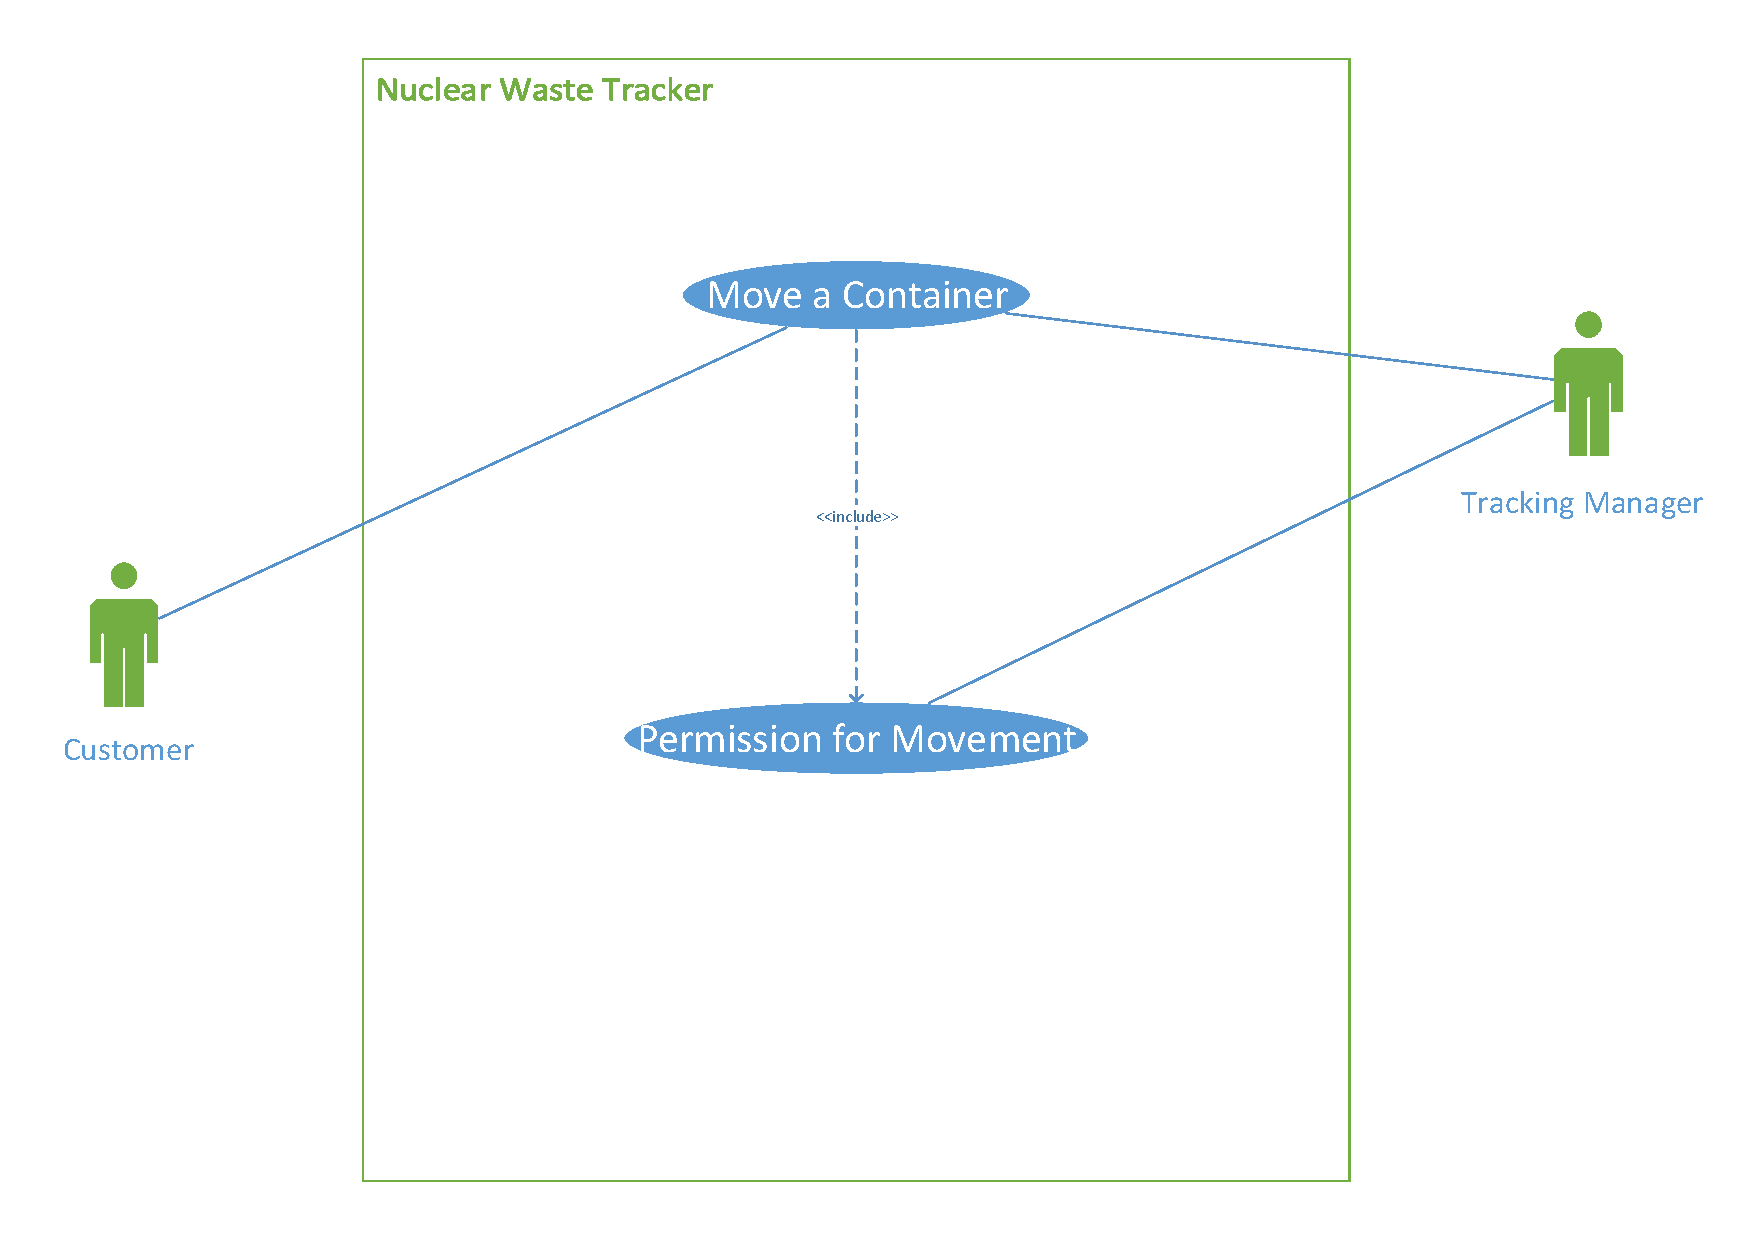
\includegraphics[width=.9\textwidth]{images/move_container_uc.pdf}
\end{center}
\caption{Use Case Diagram}
\label{fig:move_container_uc}
\end{figure}

\newpage
\section{Acceptance Test}
The following shows some sample user input and the output state of the tracker in an abstract manner:
\\
\begin{code}
->create_plant( 5.0, 3.0)
status: ok
phases: {}
containers: {}
->add_phase( "ph_unpack", "unpack", 2, [metal, plastic, glass])
status: ok
phases: {ph_unpack}
containers: {}
->add_phase( "ph_store", "compact", 3, [metal, glass, liquid])
status: ok
phases: {ph_unpack, ph_store}
containers: {}
->add_container("cn_1", metal, 2.0, "ph_unpack")
status: ok
phases: {ph_unpack, ph_store}
containers: {[cn_1 in ph_unpack]}
->add_container("cn_2", liquid, 2.0, "ph_unpack")
status: ERROR: material cannot be treated in this phase
phases: {ph_unpack, ph_store}
containers: {[cn_1 in ph_unpack]}
->add_container("cn_2", liquid, 2.0, "ph_store")
status: ok
phases: {ph_unpack, ph_store}
containers: {[cn_1 in ph_unpack], [cn_2 in ph_store]}
->add_container("cn_3", glass, 2.0, "ph_store")
status: ok
phases: {ph_unpack, ph_store}
containers: {[cn_1 in ph_unpack], [cn_2 in ph_store],
                  [cn_3 in ph_store]}
->move_container("cn_1", "ph_store")
status: ERROR:  phase radiation exceeds limit
phases: {ph_unpack, ph_store}
containers: {[cn_1 in ph_unpack], [cn_2 in ph_store], 
	             [cn_3 in ph_store]}
->move_container("cn_3", "ph_unpack")
status: ok
phases: {ph_unpack, ph_store}
containers: {[cn_1 in ph_unpack], [cn_2 in ph_store], 
                  [cn_3 in ph_unpack]}
->add_phase( "ph_clean", "compact", 3, [metal, glass, plastic])
status: ok
phases: {ph_unpack, ph_store, ph_clean}
containers: {[cn_1 in ph_unpack], [cn_2 in ph_store], 
                  [cn_3 in ph_unpack]}
->remove_phase( "ph_clean")
status: ok
phases: {ph_unpack, ph_store}
containers: {[cn_1 in ph_unpack], [cn_2 in ph_store], 
                  [cn_3 in ph_unpack]}
->add_container("cn_4", metal, 1.0, "ph_unpack")
status: ERROR: no more containers allowed in phase
phases: {ph_unpack, ph_store}
containers: {[cn_1 in ph_unpack], [cn_2 in ph_store], 
                  [cn_3 in ph_unpack]}
->add_container("cn_4", metal, 1.0, "ph_store")
status: ok
phases: {ph_unpack, ph_store}
containers: {[cn_1 in ph_unpack], [cn_2 in ph_store], 
                  [cn_3 in ph_unpack], [cn_4 in ph_store]}
\end{code}

\newpage
\section{Safety Invariant}
One important invariant is to make sure that all phases and containers have a radiation that is less than the maximum amount of radiation allowed in a container and phase as specified in the plant ($mc\_radiation$ and $mp\_radiation$). This is a way to ensure that care is taken to prevent too much build up of dangerous materials in a phase. \\ \\

\begin{mdframed}
$SafeRadiationAmount: \forall c \in CONTAINERS, p \in PHASES: \\ c.radiation <= mc\_radiation \land p.radiation <= mp\_radiation$
\end{mdframed}

\end{document}  